\documentclass[12pt]{article}


\usepackage{amssymb}
\usepackage{amsmath}
\usepackage{fullpage}
\usepackage{epsfig}
\usepackage{epstopdf}
\everymath{\displaystyle}



\begin{document}

\begin{center}
\underline{\LARGE{Chapter 1.1 Practice Problems}}
\end{center}

EXPECTED SKILLS:

\begin{itemize}

\item Given the graph of a function $y=f(x)$, be able to determine the limit of $f(x)$ as $x$ approaches some finite value (as both a one-sided and two-sided limit).

\item Know how to determine when such a limit does not exist, and if appropriate, indicate whether the behavior of the function increases or decreases without bound.

\end{itemize}

PRACTICE PROBLEMS:

{\bf Questions 1-5 refer to the function $F(x)$, which is illustrated below.}

\begin{center}
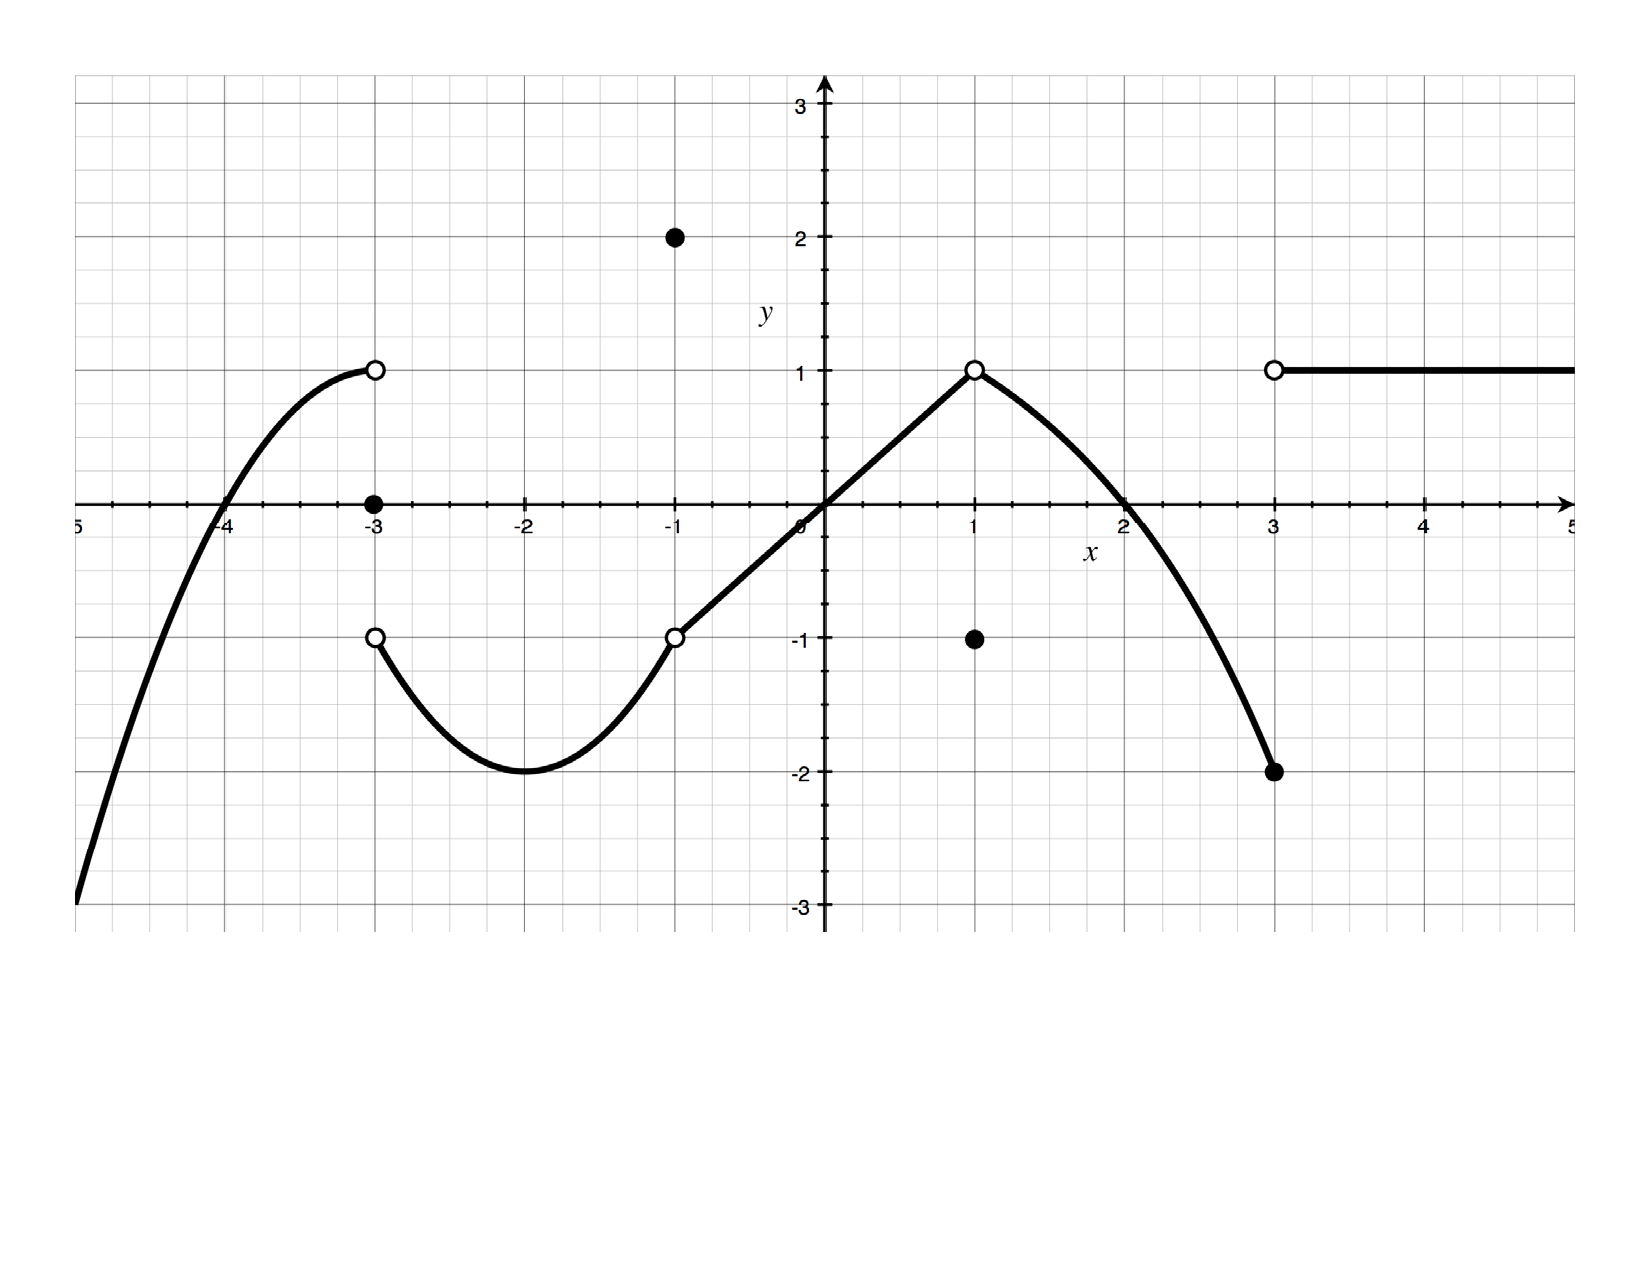
\includegraphics[scale=0.5]{Limits1.pdf}
\end{center}

\begin{enumerate}

\item Compute each of the following quantities.  If a limit does not exist, write $+\infty$, $-\infty$, or DNE (whichever is most appropriate). 

\begin{enumerate}

\item $\displaystyle \lim_{x \rightarrow 1^{-}}{F(x)}$

\includegraphics[scale=0.5]{start.pdf}
{{1}}
\includegraphics[scale=0.5]{end.pdf}


\item $\displaystyle \lim_{x \rightarrow 1^{+}}{F(x)}$

\includegraphics[scale=0.5]{start.pdf}
{{1}}
\includegraphics[scale=0.5]{end.pdf}


\item $\displaystyle \lim_{x \rightarrow 1}{F(x)}$

\includegraphics[scale=0.5]{start.pdf}
{{1}}
\includegraphics[scale=0.5]{end.pdf}


\item $F(1)$

\includegraphics[scale=0.5]{start.pdf}
{{$-1$}}
\includegraphics[scale=0.5]{end.pdf}


\end{enumerate}

\newpage

\item Compute each of the following quantities.  If a limit does not exist, write $+\infty$, $-\infty$, or DNE (whichever is most appropriate). 

\begin{enumerate}

\item $\displaystyle \lim_{x \rightarrow 3^{-}}{F(x)}$

\includegraphics[scale=0.5]{start.pdf}
{{$-2$}}
\includegraphics[scale=0.5]{end.pdf}


\item $\displaystyle \lim_{x \rightarrow 3^{+}}{F(x)}$

\includegraphics[scale=0.5]{start.pdf}
{{$1$}}
\includegraphics[scale=0.5]{end.pdf}


\item $\displaystyle \lim_{x \rightarrow 3}{F(x)}$

\includegraphics[scale=0.5]{start.pdf}
{{DNE because $\displaystyle \lim_{x \rightarrow 3^{-}}{F(x)} \neq \lim_{x \rightarrow 3^{+}}{F(x)}$}}
\includegraphics[scale=0.5]{end.pdf}


\item $F(3)$

\includegraphics[scale=0.5]{start.pdf}
{{$-2$}}
\includegraphics[scale=0.5]{end.pdf}


\end{enumerate}

\item Compute each of the following quantities.  If a limit does not exist, write $+\infty$, $-\infty$, or DNE (whichever is most appropriate). 

\begin{enumerate}

\item $\displaystyle \lim_{x \rightarrow 0^{-}}{F(x)}$

\includegraphics[scale=0.5]{start.pdf}
{{$0$}}
\includegraphics[scale=0.5]{end.pdf}


\item $\displaystyle \lim_{x \rightarrow 0^{+}}{F(x)}$

\includegraphics[scale=0.5]{start.pdf}
{{$0$}}
\includegraphics[scale=0.5]{end.pdf}


\item $\displaystyle \lim_{x \rightarrow 0}{F(x)}$

\includegraphics[scale=0.5]{start.pdf}
{{$0$}}
\includegraphics[scale=0.5]{end.pdf}


\item $F(0)$

\includegraphics[scale=0.5]{start.pdf}
{{$0$}}
\includegraphics[scale=0.5]{end.pdf}


\end{enumerate}

\item Compute each of the following quantities.  If a limit does not exist, write $+\infty$, $-\infty$, or DNE (whichever is most appropriate). 

\begin{enumerate}

\item $\displaystyle \lim_{x \rightarrow -1^{-}}{F(x)}$

\includegraphics[scale=0.5]{start.pdf}
{{$-1$}}
\includegraphics[scale=0.5]{end.pdf}


\item $\displaystyle \lim_{x \rightarrow -1^{+}}{F(x)}$

\includegraphics[scale=0.5]{start.pdf}
{{$-1$}}
\includegraphics[scale=0.5]{end.pdf}


\item $\displaystyle \lim_{x \rightarrow -1}{F(x)}$

\includegraphics[scale=0.5]{start.pdf}
{{$-1$}}
\includegraphics[scale=0.5]{end.pdf}


\item $F(-1)$

\includegraphics[scale=0.5]{start.pdf}
{{$2$}}
\includegraphics[scale=0.5]{end.pdf}


\end{enumerate}

\item Compute each of the following quantities.  If a limit does not exist, write $+\infty$, $-\infty$, or DNE (whichever is most appropriate). 

\begin{enumerate}

\item $\displaystyle \lim_{x \rightarrow -3^{-}}{F(x)}$

\includegraphics[scale=0.5]{start.pdf}
{{$1$}}
\includegraphics[scale=0.5]{end.pdf}


\item $\displaystyle \lim_{x \rightarrow -3^{+}}{F(x)}$

\includegraphics[scale=0.5]{start.pdf}
{{$-1$}}
\includegraphics[scale=0.5]{end.pdf}


\item $\displaystyle \lim_{x \rightarrow -3}{F(x)}$

\includegraphics[scale=0.5]{start.pdf}
{{DNE because $\displaystyle \lim_{x \rightarrow -3^{-}}{F(x)} \neq \lim_{x \rightarrow -3^{+}}{F(x)}$}}
\includegraphics[scale=0.5]{end.pdf}


\item $F(-3)$

\includegraphics[scale=0.5]{start.pdf}
{{$0$}}
\includegraphics[scale=0.5]{end.pdf}


\end{enumerate}

\end{enumerate}

\newpage

{\bf Questions 6-9 refer to the graph of $G(x)$, which is illustrated below.}

\begin{center}
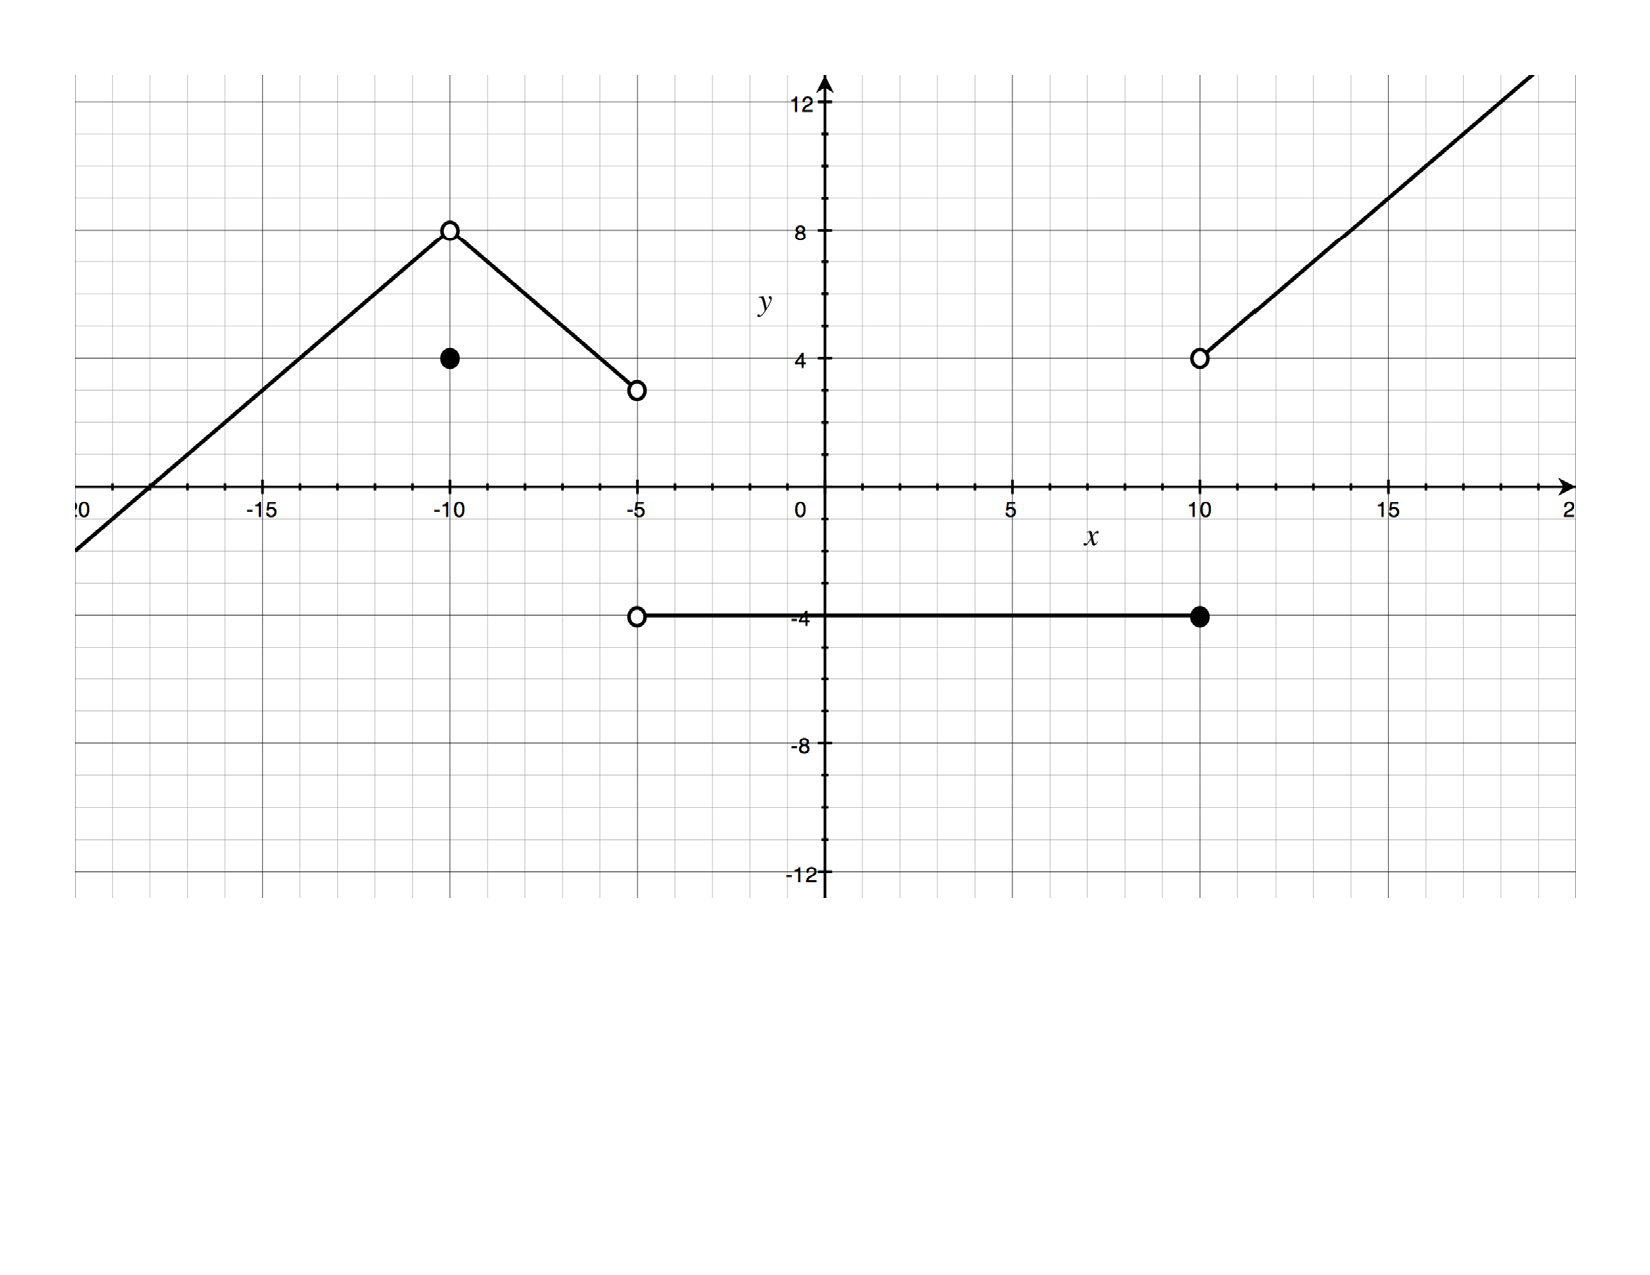
\includegraphics[scale=0.5]{Limits2.pdf}
\end{center}

\begin{enumerate}
\setcounter{enumi}{5}

\item Compute each of the following quantities.  If a limit does not exist, write $+\infty$, $-\infty$, or DNE (whichever is most appropriate). 

\begin{enumerate}

\item $\displaystyle \lim_{x \rightarrow -10^{-}}{G(x)}$

\includegraphics[scale=0.5]{start.pdf}
{{$8$}}
\includegraphics[scale=0.5]{end.pdf}


\item $\displaystyle \lim_{x \rightarrow -10^{+}}{G(x)}$

\includegraphics[scale=0.5]{start.pdf}
{{$8$}}
\includegraphics[scale=0.5]{end.pdf}


\item $\displaystyle \lim_{x \rightarrow -10}{G(x)}$

\includegraphics[scale=0.5]{start.pdf}
{{$8$}}
\includegraphics[scale=0.5]{end.pdf}


\item $G(-10)$

\includegraphics[scale=0.5]{start.pdf}
{{$4$}}
\includegraphics[scale=0.5]{end.pdf}


\end{enumerate}

\item Compute each of the following quantities.  If a limit does not exist, write $+\infty$, $-\infty$, or DNE (whichever is most appropriate). 

\begin{enumerate}

\item $\displaystyle \lim_{x \rightarrow -5^{-}}{G(x)}$

\includegraphics[scale=0.5]{start.pdf}
{{$3$}}
\includegraphics[scale=0.5]{end.pdf}


\item $\displaystyle \lim_{x \rightarrow -5^{+}}{G(x)}$

\includegraphics[scale=0.5]{start.pdf}
{{$-4$}}
\includegraphics[scale=0.5]{end.pdf}


\item $\displaystyle \lim_{x \rightarrow -5}{G(x)}$

\includegraphics[scale=0.5]{start.pdf}
{{DNE because $\displaystyle \lim_{x \rightarrow -5^{-}}{G(x)} \neq \lim_{x \rightarrow -5^{+}}{G(x)}$}}
\includegraphics[scale=0.5]{end.pdf}


\item $G(-5)$

\includegraphics[scale=0.5]{start.pdf}
{{Undefined}}
\includegraphics[scale=0.5]{end.pdf}


\end{enumerate}

\item Compute each of the following quantities.  If a limit does not exist, write $+\infty$, $-\infty$, or DNE (whichever is most appropriate). 

\begin{enumerate}

\item $\displaystyle \lim_{x \rightarrow 0^{-}}{G(x)}$

\includegraphics[scale=0.5]{start.pdf}
{{$-4$}}
\includegraphics[scale=0.5]{end.pdf}


\item $\displaystyle \lim_{x \rightarrow 0^{+}}{G(x)}$

\includegraphics[scale=0.5]{start.pdf}
{{$-4$}}
\includegraphics[scale=0.5]{end.pdf}


\item $\displaystyle \lim_{x \rightarrow 0}{G(x)}$

\includegraphics[scale=0.5]{start.pdf}
{{$-4$}}
\includegraphics[scale=0.5]{end.pdf}


\item $G(0)$

\includegraphics[scale=0.5]{start.pdf}
{{$-4$}}
\includegraphics[scale=0.5]{end.pdf}


\end{enumerate}

\newpage

\item Compute each of the following quantities.  If a limit does not exist, write $+\infty$, $-\infty$, or DNE (whichever is most appropriate). 

\begin{enumerate}

\item $\displaystyle \lim_{x \rightarrow 10^{-}}{G(x)}$

\includegraphics[scale=0.5]{start.pdf}
{{$-4$}}
\includegraphics[scale=0.5]{end.pdf}


\item $\displaystyle \lim_{x \rightarrow 10^{+}}{G(x)}$

\includegraphics[scale=0.5]{start.pdf}
{{$4$}}
\includegraphics[scale=0.5]{end.pdf}


\item $\displaystyle \lim_{x \rightarrow 10}{G(x)}$

\includegraphics[scale=0.5]{start.pdf}
{{DNE because $\displaystyle \lim_{x \rightarrow 10^{-}}{G(x)} \neq \lim_{x \rightarrow 10^{+}}{G(x)}$}}
\includegraphics[scale=0.5]{end.pdf}


\item $G(10)$

\includegraphics[scale=0.5]{start.pdf}
{{$-4$}}
\includegraphics[scale=0.5]{end.pdf}


\end{enumerate}

\end{enumerate}

{\bf Questions 10-12 refer to the graph of $H(x)$, which is illustrated below.}

\begin{center}
\includegraphics[scale=0.5]{Limits3.pdf}
\end{center}

\begin{enumerate}
\setcounter{enumi}{9}

\item Compute each of the following quantities.  If a limit does not exist, write $+\infty$, $-\infty$, or DNE (whichever is most appropriate). 

\begin{enumerate}

\item $\displaystyle \lim_{x \rightarrow -2^{-}}{H(x)}$

\includegraphics[scale=0.5]{start.pdf}
{{$1$}}
\includegraphics[scale=0.5]{end.pdf}


\item $\displaystyle \lim_{x \rightarrow -2^{+}}{H(x)}$

\includegraphics[scale=0.5]{start.pdf}
{{$+\infty$}}
\includegraphics[scale=0.5]{end.pdf}


\item $\displaystyle \lim_{x \rightarrow -2}{H(x)}$

\includegraphics[scale=0.5]{start.pdf}
{{DNE}}
\includegraphics[scale=0.5]{end.pdf}


\item $H(-2)$

\includegraphics[scale=0.5]{start.pdf}
{{Undefined}}
\includegraphics[scale=0.5]{end.pdf}


\end{enumerate}

\item Compute each of the following quantities.  If a limit does not exist, write $+\infty$, $-\infty$, or DNE (whichever is most appropriate). 

\begin{enumerate}

\item $\displaystyle \lim_{x \rightarrow 0^{-}}{H(x)}$

\includegraphics[scale=0.5]{start.pdf}
{{$-\infty$}}
\includegraphics[scale=0.5]{end.pdf}


\item $\displaystyle \lim_{x \rightarrow 0^{+}}{H(x)}$

\includegraphics[scale=0.5]{start.pdf}
{{$-1$}}
\includegraphics[scale=0.5]{end.pdf}


\item $\displaystyle \lim_{x \rightarrow 0}{H(x)}$

\includegraphics[scale=0.5]{start.pdf}
{{DNE}}
\includegraphics[scale=0.5]{end.pdf}


\item $H(0)$

\includegraphics[scale=0.5]{start.pdf}
{{$1$}}
\includegraphics[scale=0.5]{end.pdf}


\end{enumerate}

\item Compute each of the following quantities.  If a limit does not exist, write $+\infty$, $-\infty$, or DNE (whichever is most appropriate). 

\begin{enumerate}

\item $\displaystyle \lim_{x \rightarrow 2^{-}}{H(x)}$

\includegraphics[scale=0.5]{start.pdf}
{{$-1$}}
\includegraphics[scale=0.5]{end.pdf}


\item $\displaystyle \lim_{x \rightarrow 2^{+}}{H(x)}$

\includegraphics[scale=0.5]{start.pdf}
{{$-1$}}
\includegraphics[scale=0.5]{end.pdf}


\item $\displaystyle \lim_{x \rightarrow 2}{H(x)}$

\includegraphics[scale=0.5]{start.pdf}
{{$-1$}}
\includegraphics[scale=0.5]{end.pdf}


\item $H(2)$

\includegraphics[scale=0.5]{start.pdf}
{{$-1$}}
\includegraphics[scale=0.5]{end.pdf}


\end{enumerate}

\item Let $\displaystyle f(x)=\left\{ 
\begin{array}{lll}
2-x & \text{if} & x < 0\\
6-x^2& \text{if} & 0<x<3 \\
x-6 & \text{if} & x \geq 3
\end{array}\right.$\\
Sketch the graph of $f(x)$ and use your graph to compute each of the following:\includegraphics[scale=0.5]{start.pdf}
{\\}
\includegraphics[scale=0.5]{end.pdf}


\includegraphics[scale=0.5]{start.pdf}
{{\includegraphics[scale=0.5]{graph.pdf}}}
\includegraphics[scale=0.5]{end.pdf}


\begin{enumerate}

\item $\displaystyle \lim_{x \rightarrow 0^{-}}{f(x)}$

\includegraphics[scale=0.5]{start.pdf}
{{$2$}}
\includegraphics[scale=0.5]{end.pdf}


\item $\displaystyle \lim_{x \rightarrow 0^{+}}{f(x)}$

\includegraphics[scale=0.5]{start.pdf}
{{$6$}}
\includegraphics[scale=0.5]{end.pdf}


\item $\displaystyle \lim_{x \rightarrow 0}{f(x)}$

\includegraphics[scale=0.5]{start.pdf}
{{DNE because $\displaystyle \lim_{x \rightarrow 0^{-}}f(x) \neq \lim_{x \rightarrow 0^{+}}f(x)$}}
\includegraphics[scale=0.5]{end.pdf}


\item $f(0)$

\includegraphics[scale=0.5]{start.pdf}
{{Undefined}}
\includegraphics[scale=0.5]{end.pdf}


\item $\displaystyle \lim_{x \rightarrow 3^{-}}{f(x)}$

\includegraphics[scale=0.5]{start.pdf}
{{$-3$}}
\includegraphics[scale=0.5]{end.pdf}


\item $\displaystyle \lim_{x \rightarrow 3^{+}}{f(x)}$

\includegraphics[scale=0.5]{start.pdf}
{{$-3$}}
\includegraphics[scale=0.5]{end.pdf}


\item $\displaystyle \lim_{x \rightarrow 3}{f(x)}$

\includegraphics[scale=0.5]{start.pdf}
{{$-3$}}
\includegraphics[scale=0.5]{end.pdf}


\item $f(3)$

\includegraphics[scale=0.5]{start.pdf}
{{$-3$}}
\includegraphics[scale=0.5]{end.pdf}


\end{enumerate}

\item Sketch the graph of a function $y=f(x)$ which satisfies the following conditions. (There are many possible answers.)

\begin{itemize}

\item The domain is $(-1,2]$.

\item $f(1)=f(2)=5$

\item $\displaystyle \lim_{x\rightarrow 1^{-}}{f(x)}=4$

\item $\displaystyle \lim_{x\rightarrow -1^{+}}{f(x)}=-\infty$

\end{itemize}

\includegraphics[scale=0.5]{start.pdf}
{{\includegraphics[scale=0.4]{graph2}}}
\includegraphics[scale=0.5]{end.pdf}


\newpage

\item Sketch the graph of a function $y=f(x)$ which satisfies the following conditions. (There are many possible answers.)

\begin{itemize}

\item $f(-x)=-f(x)$

\item $\displaystyle \lim_{x\rightarrow 0^{+}}{f(x)}=+\infty$

\item $\displaystyle \lim_{x\rightarrow 1^{-}}{f(x)}=4$

\item $\displaystyle \lim_{x \rightarrow 6^{-}}{f(x)} \neq \lim_{x \rightarrow 6^{+}}{f(x)}$ .

\end{itemize}

\includegraphics[scale=0.5]{start.pdf}
{{\includegraphics[scale=0.4]{graph3.pdf}}}
\includegraphics[scale=0.5]{end.pdf}


\item For each of the following, determine whether the given statement is true or false.  If the statement is false, give a specific counterexample.

\begin{enumerate}

\item If $f(x)$ is not defined at $x=c$, then $\lim_{x\rightarrow c}f(x)$ DNE.

\includegraphics[scale=0.5]{start.pdf}
{{{1\linewidth}{False.  For example, consider $f(x)=\left\{\begin{array}{ll}
1 & \text{if } x<0\\
1 & \text{if } x>0\end{array}\right.$.  Then, even though $f(0)$ is undefined, we have $\lim_{x\rightarrow 0}f(x)=1$.}}}
\includegraphics[scale=0.5]{end.pdf}


\item If $\lim_{x\rightarrow a^-}f(x)=L$, then $\lim_{x\rightarrow a}f(x)=L$.

\includegraphics[scale=0.5]{start.pdf}
{{{1\linewidth}{False.  For example, consider $f(x)=\left\{\begin{array}{ll}
1 & \text{if } x<0\\
2 & \text{if } x>0\end{array}\right.$.  Then, $\lim_{x\rightarrow 0^-}f(x)=1$; but, $\lim_{x\rightarrow 0}f(x)$ DNE because $\lim_{x\rightarrow 0^+}f(x)=2\neq1$.}}}
\includegraphics[scale=0.5]{end.pdf}


\end{enumerate}

\end{enumerate}

\end{document}